\chapter{Data basis}
\label{chap:data_basis}

The previous chapter mentioned quantifying runoff and parameters affecting hydroelectricity production. In this chapter, the data sets used in this work will be described and analyzed. This include power plants data registers and production data, as well as runoff data sets.

\section{Hydroelectricity}
\label{hpp_register}

\subsection{Power plant register}
\label{sub:hpp_reg}
This work, as well as the project open\_FRED, is linked to the OpenEnergy Platform, developed by the Reiner Lemoine Institute within the open\_eGo project. The OpenEnergy Platform provides necessary tools for transparent and collaborative energy system modeling \cite{oedb}, such as grid data, power plants register, geography data or weather data. The OpenEnergy Database has 7491 entries for run-of-the-river hydropower plants in Germany and contains, among others, the following information :
\begin{itemize}
\itemsep0em 
 \item EEG ID
 \item Company operating the plant
 \item Adress and state
 \item Startup, retrofit and shutdown years
 \item Electrical capacity [\unit{MW}]
 \item Network operator information
 \item Position (latitude, longitude, and GIS geometry)
\end{itemize}


Figure \ref{oedb_capa} shows the repartition of the capacity of these plants. This is consistent with the Umweltbundesamt numbers of 6500 to 7500 hydropower plants excluding pumped hydro, among which 406 with a nominal power above \unit[1]{MW} \cite{uba_wasserkraft}. 

\begin{figure}[H]
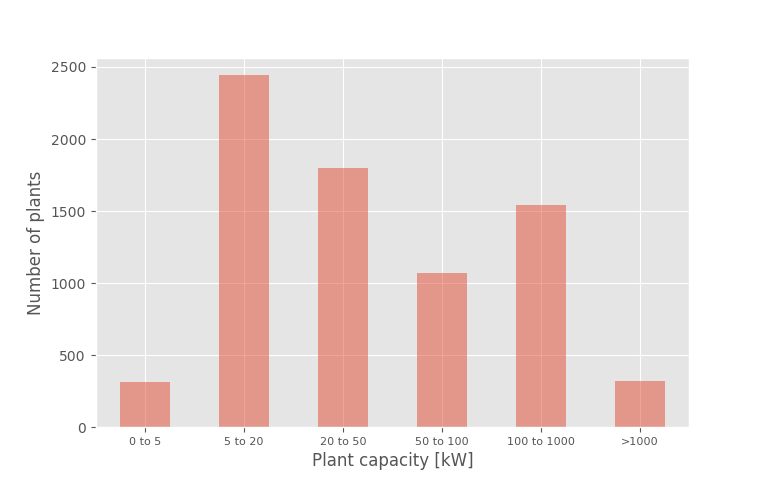
\includegraphics[width=15cm]{oedb_capa.png}
\caption[Repartition of the capacity of run-of-the-river plants in the OpenEnergy Database]{Repartition of the capacity of run-of-the-river plants plants in the OpenEnergy Database}
\centering
\label{oedb_capa}
\end{figure}

The OpenEnergy Database also has entries for reservoir and pumped storage plants, listed in table \ref{oedb_pump_res}.

\begin{table}
\footnotesize
  \caption[Number of plants and installed capacity per federal state - reservoir and pumped storage plants]{Number of plants and installed capacity per federal state - reservoir and pumped storage plants \cite{oedb}}
  \centering
  \label{oedb_pump_res}
  \begin{tabular}{|c|cc|cc| }
  \cline{2-5}
  \multicolumn{0}{c|}{} &\multicolumn{2}{|c}{\textbf{Reservoir plants}}&\multicolumn{2}{|c|}{\textbf{Pumped storage plants}} \\
  \hline
  \textbf{State} & Number 	& 	Capacity [\unit{MW}] 	&	Number 	& 	Capacity [\unit{MW}] 	 \\
  \hline
  SH	&	0	&	0		&	3	&	119.1	\\
  NI	&	0	&	0		&	1	&	220	\\
  NRW	&	1	&	15		&	2	&	291	\\
  HE	&	2	&	40		&	2	&	623	\\
  BW	&	0	&	0		&	7	&	1873	\\	
  BY	&	2	&	169.5		&	7	&	587	\\
  SN	&	0	&	0		&	8	&	1085	\\
  ST	&	0	&	0		&	2	&	79.7	\\
  TH	&	0	&	0		&	16	&	1509.4	\\
  \hline
  \end{tabular}
\end{table}

\subsection{Capacity and production data}
\label{sub:prod_data}

The Agentur für Erneuerbare Energien (AEE) provides data about the installed capacity, electricity generation over the year and number of hydropower plants for each federal state \cite{aee} from 2001 to 2014 (based on data from the Bundesverband der Energie- und Wasserwirtschaft). This data contains run-of-the-river and reservoir plants, as well as pumped storage power plants with natural inflow for which only the production from natural inflow is accounted for. Therefore, it might show discrepancies with the OEDB register for run-of-the-river plants. Table \ref{oedb_aee_diff} lists the number of plants and installed capacity per federal state from these two sources, as well as the relative difference for each state, with the AEE data as reference. The OEDB entries for pumped storage and reservoir plants, listed in table \ref{oedb_pump_res} were not used in this work because they cannot be simulated with the developed model. Moreover, these data do not make up for the difference between the OEDB and the AEE shown in table \ref{oedb_aee_diff} and figures \ref{map_diff_num} and \ref{map_diff_pow}, and the pumped storage entries from the OEDB do not make the distinction between natural inflow and pumped inflow.

\begin{table}
\footnotesize 
 \caption[Number of hydropower plants and installed capacity per federal state]{Number of hydropower plants and installed capacity per federal state}
 \centering
 \label{oedb_aee_diff}
 \begin{tabular}{|c|cc|cc| cc|}
  \cline{2-7}
  \multicolumn{0}{c|}{} &\multicolumn{2}{|c}{\textbf{OEDB \cite{oedb}}}&\multicolumn{2}{|c|}{\textbf{AEE \cite{aee}}}&\multicolumn{2}{c|}{\textbf{Difference}} \\
  \hline
  \textbf{State} & Number 	& 	Capacity [\unit{MW}] 	&	Number 	& 	Capacity [\unit{MW}] 	&	Number [\unit{\%}] 	&	Capacity [\unit{\%}] \\
  \hline
  SH	&	29	&	8.1		&	24	&	5		&	20.8		&	62.8	\\
  HH	&	1	&	0.11		&	1	&	0.1		&	0		&	10	\\
  NI	&	258	&	56.3		&	257	&	70		&	0.4		&	-19	\\
  HB	&	1	&	10		&	1	&	10		&	0		&	0	\\
  NRW	&	437	&	137.8		&	409	&	202		&	6.9		&	-31.8	\\
  HE	&	463	&	51.9		&	482	&	82		&	-3.9		&	-36.7	\\
  RLP	&	217	&	40.8		&	199	&	218		&	9		&	-81.3	\\
  BW	&	1741	&	464.5		&	1485	&	960		&	17		&	-51.6	\\	
  BY	&	3657	&	666.2		&	3578	&	2661		&	2.2		&	-75	\\
  SL	&	26	&	11.1		&	26	&	24		&	0		&	-53.6	\\
  B	&	0	&	0		&	0	&	0		&	0		&	0	\\
  BB	&	42	&	5.3		&	38	&	6		&	10.5		&	-11.8	\\
  MV	&	25	&	3		&	24	&	3		&	4.2		&	-0.1	\\
  SN	&	322	&	134.4		&	330	&	99		&	-2.4		&	35.8	\\
  ST	&	57	&	26		&	52	&	26		&	9.6		&	0.2	\\
  TH	&	204	&	32.6		&	198	&	32		&	3		&	2	\\
  \hline
 \end{tabular} 
\end{table}




The relative difference is shown on figures \ref{map_diff_num} and \ref{map_diff_pow}, which respectively display the differences in the number of plants and in the installed capacity. The analysis of these two maps and of table \ref{oedb_aee_diff} shows that the OEDB and AEE databases are consistent in three federal state : Thuringia, Saxony-Anhalt and Mecklenburg-Vorpommern (Berlin and Bremen being excluded due to the near absence of hydropower). The discrepancies in other federal states can be explained by different reasons. First, the data of the the AEE are based on all hydropower plants, including reservoir plants and natural inflow in pumped storage plants. This is why both the number of plants and the installed capacity are greater in the AEE data for most states. Second, these reservoir plants and pumped storage plants tend to have a bigger capacity than most run-of-the-river plants, which explains that the difference in installed capacity is not proportional to the difference in number of plants. Finally, rivers often mark boundaries between states and countries, and some hydropower plant are operated by two countries or inject electricity into the grids of more than one country. It is possible that the AEE and the OEDB don't count the installed capacity in the same manner in this situation. Figure \ref{map_diff_pow} shows a bigger discrepancy in installed capacity for border states.


\begin{figure}[H]
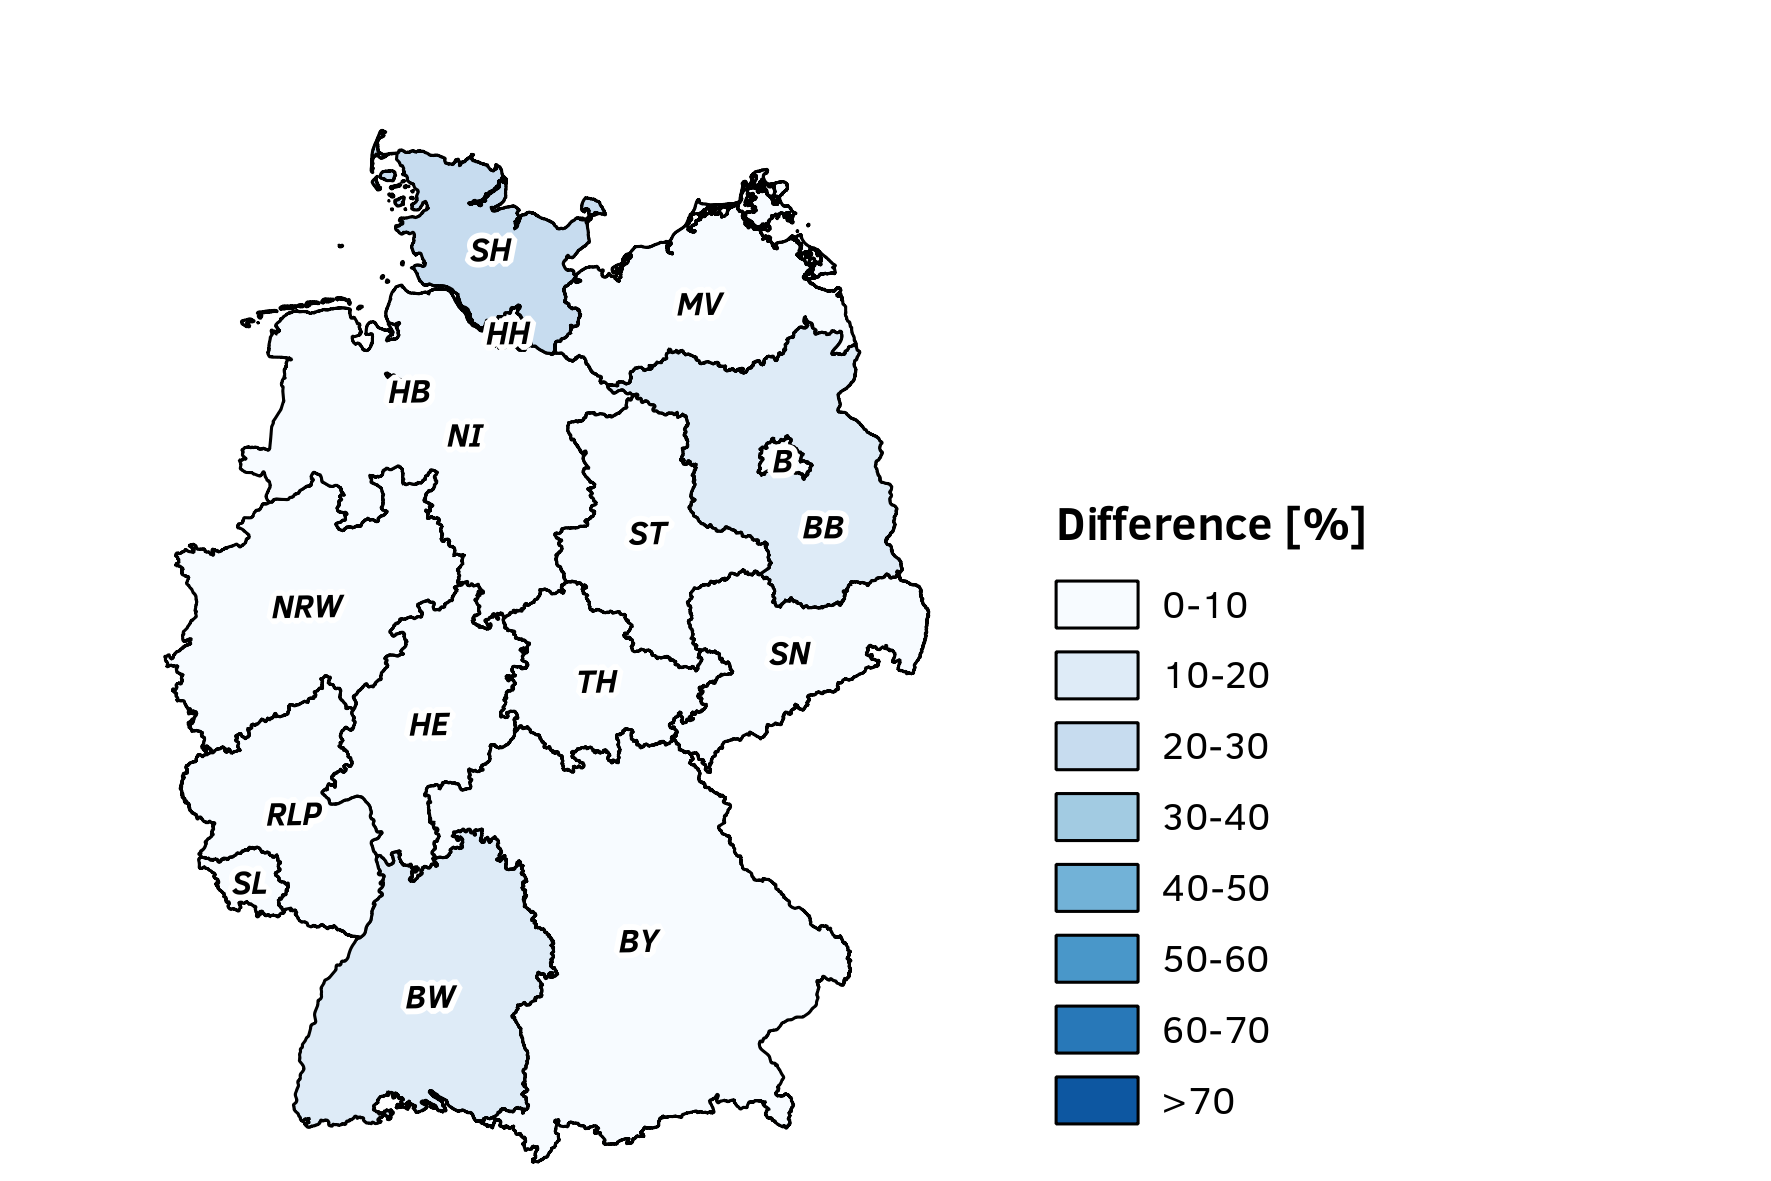
\includegraphics[width=15cm]{map_diff_num.png}
\caption[Absolute difference in the number of plants between OEDB and AEE]{Absolute difference in the number of plants between OEDB and AEE}
\centering
\label{map_diff_num}
\end{figure}


\begin{figure}[H]
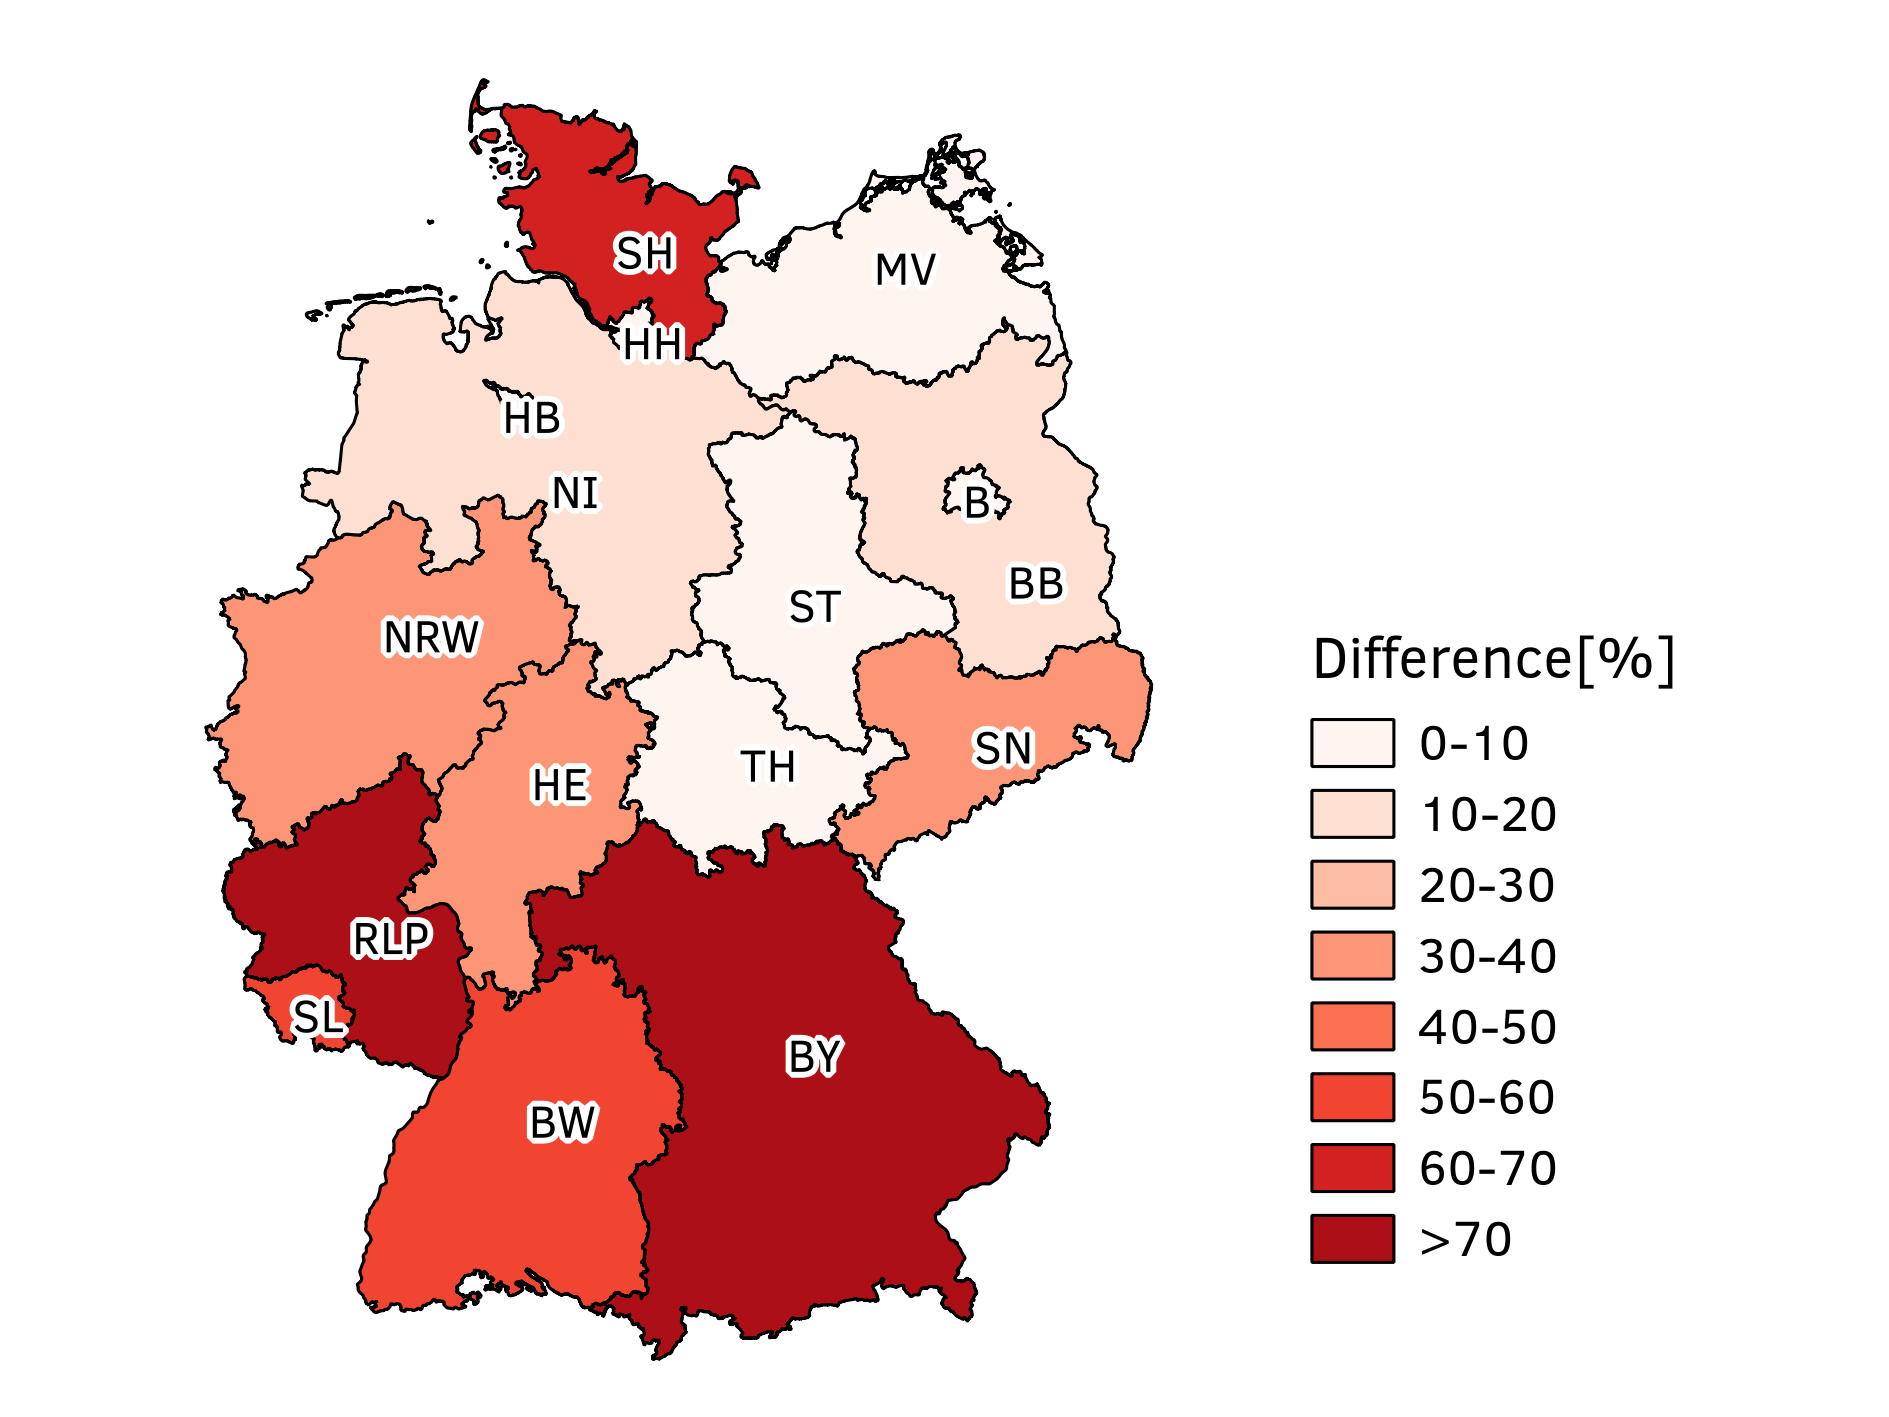
\includegraphics[width=15cm]{map_diff_pow.png}
\caption[Absolute difference in the installed capacity between OEDB and AEE]{Absolute difference in the installed capacity between OEDB and AEE}
\centering
\label{map_diff_pow}
\end{figure}

\section{Runoff data - measured}

\label{meas_runoff}
Water levels and water flows of the main rivers are regularly measured and documented by several organizations, in order to keep track of the history of the waterways and to anticipate potential floods. In Germany, the German Federal Institute of Hydrology (Bundesanstalt für Gewässerkunde – BfG), is a supreme federal agency within the portfolio of the Federal Ministry of Transport and Digital Infrastructure. As such it is the federal government's scientific institution for research, assessments, and consulting in the fields of hydrology, uses, quality and conservation of waters and ecology \cite{bafg}. The BfG gathers data about water levels and water flows since its founding in 1949 and publishes it every year in the ``Deutsches Gewässerkundliches Jahrbuch'' (DGJ). The BfG also operates the HYDABA database, in which times series for water flow and water level are stored, going back to 1816 for daily values and 1981 for hourly values. This database gathers water levels from around 600 gauges and water flows from around 250 stations. The data can, among others, be provided to universities, public administrations, engineering or insurance companies \cite{bafg_hyd}. \newline
Another source of measured river data is Pegelonline, a service of the Federal Waterways and Shipping Administration (WSV). It publishes raw values of water levels from around 600 gauges in Germany over the previous 30 days. Some of the stations also measure water flows \cite{pegelonline}. The locations of the gauges are shown on map \ref{pegelonline}.

\begin{figure}[H]
\centering
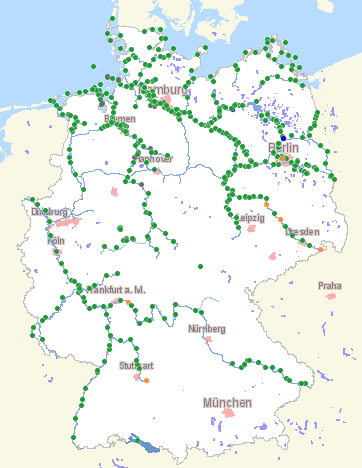
\includegraphics[width=8cm]{pegelonline.png}
\caption[Locations of the gauge stations]{Locations of the gauge stations \cite{pegelonline}}
\label{pegelonline}
\end{figure}

Other countries have similar databases for measured river data. In France, the ``Banque Hydro'' is run by the SCHAPI (Service Central d'Hydrométéorologie et d'Appui à la Prévision des Inondations), a section of the french Ministry of Ecology, Sustainable Development and Energy, and gathers and publishes data from around 5000 gauge stations.

\section{Runoff data - modeled}

Given that this work is part of the openFRED project (see ch. \ref{chap:introduction}) the runoff data should eventually be accessible from open source databases or software. A model is currently being developed by the Helmholtz Zentrum Geesthacht in partnership with the Reiner Lemoine Institute, in order to be used in the openFRED project. This model was not yet available during this work, therefore other sources where used for runoff data (see sec. XXX ref to the methodology section about measured data XXX).
